\documentclass[conference]{IEEEtran}
\IEEEoverridecommandlockouts

\usepackage{cite}
\usepackage{amsmath,amssymb,amsfonts}
\usepackage{algorithmic}
\usepackage{graphicx}
\usepackage{textcomp}
\usepackage{xcolor}
\usepackage{url}
\usepackage{booktabs}

\def\BibTeX{{\rm B\kern-.05em{\sc i\kern-.025em b}\kern-.08em
    T\kern-.1667em\lower.7ex\hbox{E}\kern-.125emX}}

\begin{document}

\title{Investigating Low-Rank Approximations for Training Pythia Models on Falcon RefinedWeb}

\author{\IEEEauthorblockN{Vyacheslav Roshchin}
\IEEEauthorblockA{\textit{FCS AMI} \\
\textit{HSE University}}
\and
\IEEEauthorblockN{Aleksandr Bolgov}
\IEEEauthorblockA{\textit{FCS AMI} \\
\textit{HSE University}}
\and
\IEEEauthorblockN{Yaroslav Vasilyev}
\IEEEauthorblockA{\textit{FCS AMI} \\
\textit{HSE University}}
}

\maketitle

\begin{abstract}
Training large language models is computationally expensive and remains one of the central challenges in modern machine learning. In this work, we study pre-training of LLama-family causal language models on the Falcon RefinedWeb dataset using validation perplexity as the primary evaluation metric. The project is primarily an empirical study: we implement and compare existing low-rank gradient projection ideas and Adam-mini-style optimizer-state reduction under one reproducible training setup.
\end{abstract}

\section{Introduction}

Large Language Models (LLMs) have shown impressive performance across multiple disciplines, including conversational AI and language translation. However, reducing memory usage during pre-training without a significant loss in quality remains an open practical challenge. Standard AdamW stores first and second optimizer moments for most trainable parameters, which becomes expensive for billion-parameter models and restricts the usable batch size on commodity GPUs.

Our project studies memory-efficient training for LLama-family models \cite{touvron2023llamaopenefficientfoundation} on the RefinedWeb corpus \cite{penedo2023refinedwebdatasetfalconllm}. We focus on low-rank gradient projection methods inspired by GaLore \cite{Galore}, GaLore 2 \cite{su2025galore2largescalellm}, and LOTUS \cite{miao2026lotusefficientllmtraining}, and on their combination with Adam-mini \cite{zhang2025adamminiusefewerlearning}. Following the feedback from the previous stage, we explicitly formulate this work as an empirical comparison rather than as a claim of a completely new optimizer family. Many components already exist in the literature; the main content of the project is to implement them under a common interface, compare them with relevant baselines, and analyze their stability in realistic pre-training runs.

The goal is to evaluate whether low-rank projection and Adam-mini can reduce memory and training cost while preserving acceptable validation perplexity. The methods are compared against AdamW, 8-bit Adam, GaLore, GaLore 2, LOTUS, GaLore-mini, GaLore 2-mini, and LOTUS-mini. Special attention is paid to instability caused by projector updates, because preliminary runs show visible loss spikes when the low-rank subspace changes during training.

\section{Related Works}

One of the most popular classical approaches to reduce memory costs is parameter-efficient fine-tuning, notably LoRA \cite{hu2022lora}. LoRA adds trainable low-rank adapters while freezing the original weights, which makes it effective for fine-tuning but unsuitable as a direct replacement for full pre-training from scratch.

GaLore \cite{Galore} applies low-rank structure to gradients instead of weights. For a matrix parameter $W \in \mathbb{R}^{m \times n}$, the gradient is projected to a rank-$r$ subspace, updated there, and reconstructed back to the original shape. This reduces optimizer-state memory from $\mathcal{O}(mn)$ to approximately $\mathcal{O}((m+n)r)$. GaLore 2 \cite{su2025galore2largescalellm} extends this direction with randomized SVD and large-scale training support.

LOTUS \cite{miao2026lotusefficientllmtraining} addresses the cost of fixed projector refreshes. Instead of recomputing the projection subspace every fixed number of steps, it tracks how efficiently the current subspace follows the gradient direction and switches the subspace adaptively. This is especially relevant for our experiments, because projector switches are one of the main sources of loss spikes.

Adam-mini \cite{zhang2025adamminiusefewerlearning} reduces optimizer memory by storing a shared second-moment estimate for parameter blocks instead of a full element-wise second moment. GaLore-mini \cite{huang2024galoremini} combines low-rank projection with Adam-mini-style memory reduction. This combination is promising, but it can be unstable because the optimizer state is maintained in compressed subspaces that change over time.

\section{Formal Problem Statement}

We consider the problem of memory-efficient optimization for causal language model pre-training. Let $D_{train}$ and $D_{val}$ denote the training and validation subsets of the RefinedWeb corpus, and let $f_\theta$ be a Pythia-family causal language model with parameters $\theta$. For a token sequence $x=(x_1,\ldots,x_T)$, the model is trained with the standard next-token prediction objective:
\[
    \ell(\theta; x) = - \sum_{t=1}^{T} \log p_\theta(x_t \mid x_{<t}).
\]
The empirical training loss is therefore
\[
    \mathcal{L}_{train}(\theta) =
    \frac{1}{|D_{train}|}
    \sum_{x \in D_{train}} \ell(\theta; x).
\]

The baseline optimization method is full-rank AdamW. The main experimental direction is to compare it with low-rank optimization approaches inspired by GaLore, LOTUS, and Adam-mini. For a matrix parameter in layer $l$, let $G_l$ be the corresponding gradient. Instead of applying the full gradient update, low-rank methods replace it with an approximation
\[
    \widehat{G}_l = \Pi_{r_l}(G_l), \qquad
    \operatorname{rank}(\widehat{G}_l) \le r_l,
\]
where $r_l$ is the selected rank and $\Pi_{r_l}$ denotes a low-rank projection based on truncated or randomized SVD.

For each optimizer configuration $\phi \in \Phi$, including the choice of rank, projection method, subspace update strategy, and optimizer variant, we train the same model from the same initialization for a fixed number of tokens or optimization steps:
\[
    \theta_T^{(\phi)} = A_\phi(\theta_0, D_{train}, T),
\]
where $A_\phi$ denotes the selected training procedure. The goal is not to obtain a state-of-the-art language model, but to study the trade-off between validation quality and computational efficiency.

\section{Evaluation Metrics}

The primary quality metric is validation perplexity. First, we compute the average validation loss
\[
    \mathcal{L}_{val}(\theta) =
    \frac{1}{|D_{val}|}
    \sum_{x \in D_{val}} \ell(\theta; x),
\]
and then define perplexity as
\[
    PPL_{val}(\theta) = \exp(\mathcal{L}_{val}(\theta)).
\]
Lower perplexity corresponds to better next-token prediction quality.

To compare low-rank methods with the baseline, we report relative perplexity degradation:
\[
    \Delta_{PPL} =
    \frac{PPL_{method} - PPL_{baseline}}
    {PPL_{baseline}}.
\]
Efficiency is evaluated using peak GPU memory consumption $M_{peak}$ and relative memory saving
\[
    S_{mem} =
    1 - \frac{M_{peak, method}}{M_{peak, baseline}}.
\]
We also measure throughput in tokens per second:
\[
    V = \frac{\text{number of processed tokens}}{\text{training time}},
\]
and relative speed change:
\[
    S_{speed} =
    \frac{V_{method}}{V_{baseline}} - 1.
\]

Finally, we record training stability. A run is considered unstable if the loss diverges, becomes NaN, or contains strong uncontrolled spikes. This is especially important for low-rank and randomized methods, since memory reduction may come at the cost of less stable optimization.

\section{Preliminary Experiments}

This section describes our part of the project. We made the training pipeline, connected the optimizer and projector code, ran first experiments, and looked at the first stability problems. These results are not final benchmark yet. They are useful mostly because they show what works and what breaks.

\subsection{Prototype Setup}

The prototype contains a RefinedWeb data loader, model wrappers, low-rank projectors, Adam-mini wrappers, and metric logging. The loader caches RefinedWeb records into local JSONL shards and packs several tokenized documents into fixed-length causal LM sequences. For packed examples it stores \texttt{position\_ids} and \texttt{sequence\_ids}; positions reset at document boundaries. This fixed an early issue where decoded batches contained long repeated end-of-text fragments instead of useful packed text.

The original target family is Pythia. During prototyping we found that the HuggingFace Pythia implementation does not provide a reliable FlashAttention path for our packed-sequence setup. Since ordinary attention materializes a large attention matrix, this became a bottleneck for large token batches. To keep testing the optimizer logic at approximately the intended scale, the current 1B-scale experiments use TinyLlama-1.1B as a decoder-only proxy with FlashAttention 2 support. The optimizer code path is the same, but these results should be treated as prototype results rather than final Pythia results.

All reported runs use cached RefinedWeb shards, rank $r=8$, batch size $16$, sequence length $2048$, and therefore $32768$ tokens per step. The learning rate is $5 \cdot 10^{-4}$, the seed is $666$, and gradient clipping with max norm $1.0$ is enabled. We record loss, a clipped perplexity proxy, peak VRAM, model memory, optimizer memory, gradient memory, activation memory, iteration time, and gradient norms. The perplexity proxy is capped at 1000, so in this first comparison we mostly look at training loss.

\subsection{Experiment Results}

\begin{table*}[t]
\caption{Preliminary experiments. All runs use Adam-mini, rank $8$, batch size $16$, sequence length $2048$, and $32768$ tokens per step.}
\label{tab:preliminary}
\centering
\begin{tabular}{lrrrrrr}
\toprule
Method & Max step & Final loss & Median loss & Min loss & Max loss & Peak VRAM \\
\midrule
GaLore-mini A & 2953 & 11.4850 & 11.4555 & 1.6492 & 32.7465 & 17.1483 GB \\
GaLore-mini B & 1974 & 2.4526 & 2.4564 & 1.7745 & 19.0123 & 17.1493 GB \\
GaLore2-mini & 1499 & 2.4794 & 2.4889 & 1.8085 & 16.3115 & 17.1493 GB \\
LOTUS-mini & 1499 & 2.4712 & 2.4836 & 1.7642 & 16.2867 & 17.1584 GB \\
\bottomrule
\end{tabular}
\end{table*}

\begin{figure}[t]
    \centering
    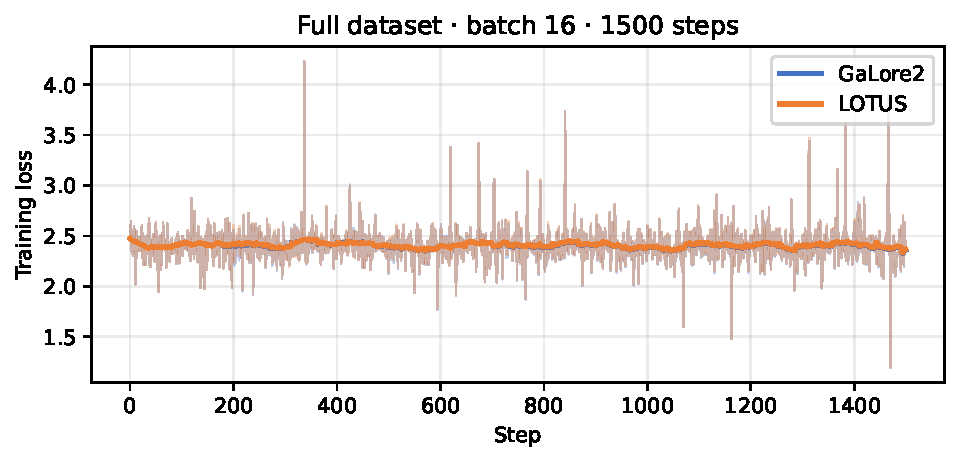
\includegraphics[width=\columnwidth]{figures/full_run/article/experiment_loss_curves.pdf}
    \caption{Training-loss curves from our experiment logs. Thin lines show raw values; thick lines show a rolling median.}
    \label{fig:comet-loss}
\end{figure}

\begin{figure}[t]
    \centering
    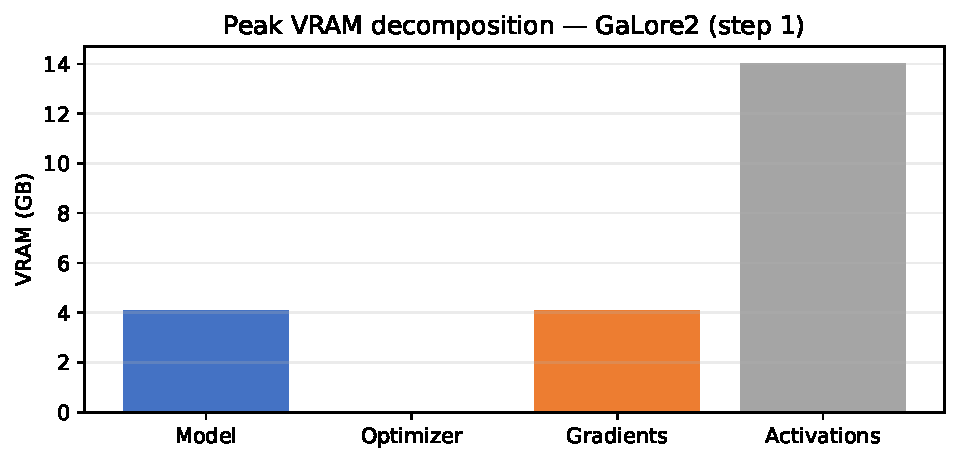
\includegraphics[width=\columnwidth]{figures/full_run/article/experiment_vram_components.pdf}
    \caption{Peak VRAM decomposition from the experiment logs. Optimizer-state memory is small compared with model, gradient, and activation memory.}
    \label{fig:comet-vram}
\end{figure}

The first small-model smoke tests showed that the pipeline can train and record metrics end to end. They also showed a problem: if we add a projector in a naive way, the loss can become NaN very fast. So we fixed the experimental setup before comparing methods. We used update gap 300 for projector refreshes, scale factor 0.25 for GaLore-style reconstruction, fixed learning rate, gradient norm logging, and clipping.

The 1.1B-scale runs show that GaLore2-mini and LOTUS-mini both reach loss around $2.47$ to $2.48$ after the same early training budget. In this prototype LOTUS-mini is a little better than GaLore2-mini in final loss and in median loss over the last recorded points. The difference is small, so we do not make strong conclusion yet. GaLore-mini looks less stable in these first runs: one curve goes down to similar loss, but another one has a big late spike.

The main observed problem is loss spikes. The first update already gives a large spike in all Adam-mini projector variants, and GaLore-mini can spike again later. Our current interpretation is simple: Adam-mini keeps optimizer state, but the low-rank subspace can change. If this state is not handled carefully, the next update may be too sharp.

\subsection{Issues Found During Experiments}

The experiments uncovered several concrete issues. First, the packed data loader had to be rewritten to avoid wasting context on repeated end-of-text padding. Second, Pythia attention support is not enough for large packed runs now, so we temporarily switched to TinyLlama-1.1B for optimizer experiments. Third, LOTUS-mini initially returned the normalized vector used for the subspace-switching criterion instead of the actual projected gradient; this caused NaNs. Fourth, when LOTUS changed the basis inside \texttt{project}, the low-rank gradient could be computed in the old basis while \texttt{reconstruct} used the new one. We fixed this by applying a pending basis update before computing the projected gradient. Finally, Adam-mini needs to reset its low-rank first moment when the projector changes basis, because the old moment lives in different coordinates.

These fixes make LOTUS-mini stable enough for the first comparison. Next we need to check the same thing with more seeds, ranks, and longer token budgets.


\section{Implemented Algorithms}
\label{sec:implemented-algorithms}

All optimizers in this study share the same Adam-mini backbone: the second moment is reduced to a single scalar per parameter matrix, while the first moment is maintained either in the original space (full-rank) or in a low-rank subspace. For a matrix parameter \(W\in\mathbb{R}^{m\times n}\) with gradient \(G\), the low-rank update proceeds as:

\[
\begin{aligned}
R &= P^\top G \quad &\text{(projection)}, \\
E &\leftarrow \beta_1 E + (1-\beta_1) R \quad &\text{(momentum in low rank)}, \\
\widehat{G} &= P E \quad &\text{(reconstruction)}.
\end{aligned}
\]

The basis \(P\in\mathbb{R}^{d_1\times r}\) (with \(d_1=\min(m,n)\)) is obtained from the singular value decomposition of \(G\) (or its randomised approximation). We compare the following projectors:

\subsection{Deterministic Baselines}
\begin{itemize}
    \item \text{GaLore-mini}: uses simple SVD to compute the top-\(r\) left singular vectors. Basis is refreshed every 300 steps.
    \item \text{GaLore2-mini}: uses randomised SVD (oversampling \(q=1\)) to compute the top-\(r\) left singular vectors. Basis is refreshed every 300 steps.
    \item \text{LOTUS-mini}: adaptively refreshes the basis based on the drift of the normalised projected gradient. When the average angular change per step drops below a threshold \(\gamma=0.05\), the basis is updated; otherwise the same basis is kept. This avoids unnecessary resets and reduces loss spikes.
\end{itemize}

\subsection{Stochastic Subspace Sampler (SSS)}
Implemented on top of LOTUS-mini. Instead of always taking the top-\(r\) singular vectors, we keep \(k_{\text{det}}=r-1\) deterministic anchors (the largest ones) and sample the remaining direction from a temperature-adjusted categorical distribution over the candidate pool. The temperature is made inversely proportional to the coefficient of variation of the singular values: flatter spectra lead to higher exploration. Low-energy and noise-floor directions are filtered out before sampling.

\subsection{Adaptive Rank Allocation}
Also built on LOTUS-mini. At each basis refresh we compute a per-layer rank \(r_{\text{adaptive}}\) from the singular value spectrum, combining an energy-based rank (98\% of variance) and an entropy-based effective rank. This allows layers with a rich spectrum to use the full \(r=8\) while nearly rank-deficient layers automatically reduce their rank, potentially saving computation.

\subsection{Fisher-Based Projectors (Diagnostic)}
We implemented two Fisher-informed projectors:
\begin{itemize}
    \item \text{Fisher projector}: accumulates the diagonal empirical Fisher \( \mathbb{E}[(u_i^\top g)^2] \) over the update window and selects the top-\(r\) directions by Fisher importance.
    \item \text{Block Fisher projector}: accumulates the full \(c\times c\) covariance \((U^\top g)(U^\top g)^\top\) in the candidate basis, diagonalises it, and rotates the basis into the Fisher eigenbasis before selecting the top-\(r\) eigenvectors.
    \item \text{Softmax / Top-k Fisher projectors}: variants that select indices either greedily (top-k) or stochastically (softmax) based on the diagonal Fisher.
\end{itemize}
These served as diagnostic tools to test whether curvature information can improve subspace selection.

\subsection{The Hybrid Optimization Step (GaLore-mini / LOTUS-mini)}
Our unified optimization step integrates low-rank gradient projection with Adam-mini state reduction. Block Fisher covariance accumulation is omitted from the core loop because it did not improve convergence in our pilot runs.

\noindent\rule[-5pt]{0.8\columnwidth}{0.4pt}
{\footnotesize
\resizebox{\columnwidth}{!}{%
\begin{minipage}{\columnwidth}
\begin{tabbing}
  \hspace{2cm}\=\hspace{2cm}\=\kill
    { Given:} Weight $W_t$, full gradient $G_t$, basis $P_t$, momentum $E_t$, scalar second moment $v_t$, learning rate $\eta$, weight decay $\lambda$, decay rates $\beta_1, \beta_2$, constant $\epsilon$. Optional flags: $\text{use\_fisher}$, $\text{use\_stochastic}$. \\*[\smallskipamount]
    1.\ Form the SVD target: $g_t = G_t$ or $g_t = G_t^T$ so that rows $\ge$ columns. \\
    2.\ Compute candidate pool: $U_{\text{pool}}, \Sigma \leftarrow \text{SVD}(g_t)$ with $\text{candidate\_rank} = c$. \\
    3.\ { if} $\text{use\_fisher} = \text{True}$ { then} \\
    \> $C \leftarrow C + (U_{\text{pool}}^T g_t)(U_{\text{pool}}^T g_t)^T / m$ \\
    4.\ { if} subspace switch is triggered { then} \\
    \> Compute $r_{\text{adaptive}}$ \\
    \> { if} $\text{use\_fisher} = \text{True}$ { then} \\
    \> \qquad \= Solve $C Q = Q \Lambda$, set $U_{\text{base}} = U_{\text{pool}} Q$ \\
    \> { else} \\
    \> \> $U_{\text{base}} = U_{\text{pool}}$ \\
    \> { if} $\text{use\_stochastic} = \text{True}$ { then} \\
    \> \> Sample $r_{\text{adaptive}}$ vectors from $U_{\text{base}}$ using $p_i \propto \exp(\sigma_i / T_{\text{temp}})$, keeping top-$k_{\text{det}}$ anchors fixed \\
    \> { else} \\
    \> \> Take top-$r_{\text{adaptive}}$ vectors from $U_{\text{base}}$ \\
    \> Form $P_t$ from the selected vectors \\
    \> $E_t \leftarrow \mathbf{0}$ \quad {(Reset momentum)} \\
    5.\ Update scalar second moment (Adam-mini): \\
    \> $v_t \leftarrow \beta_2 v_{t-1} + (1-\beta_2) \cdot {\rm mean}(G_t \odot G_t)$ \\
    6.\ Project the gradient: $R_t = P_t^T g_t$ \\
    7.\ Accumulate low-rank first moment: \\
    \> $E_t \leftarrow \beta_1 E_{t-1} + (1-\beta_1) R_t$ \\
    8.\ Reconstruct gradient update: \\
    \> $\widetilde{E}_t = \eta \cdot (P_t E_t)^T$ \quad \= { if} $g_t = G_t^T$ \\
    \> $\widetilde{E}_t = \eta \cdot (P_t E_t)$ \> { if} $g_t = G_t$ \\
    9.\ Apply decoupled weight decay: $W_t \leftarrow W_t \cdot (1 - \eta \lambda)$ \\
    10.\ Compute bias corrections and update: \\
    \> $\hat{m}_t = \widetilde{E}_t / (1 - \beta_1^t), \quad \hat{v}_t = v_t / (1 - \beta_2^t)$ \\
    \> $W_{t+1} \leftarrow W_t - \eta \cdot \frac{\hat{m}_t}{\sqrt{\hat{v}_t} + \epsilon}$
\end{tabbing}
\end{minipage}%
}
}
\noindent\rule[10pt]{0.8\columnwidth}{0.4pt}

\section{Experimental Setup}
\label{sec:experimental-setup}

Hyperparameters: learning rate \(5\times10^{-4}\) with 250-step linear warmup, weight decay 0.1, gradient clipping norm 1.0, update gap 300 (for fixed-refresh methods), LOTUS parameters \(\gamma=0.05,\ \eta=200\), rank \(r=8\) (adaptive rank clamped to \([6,8]\)). Seed 666.

\section{Results}

\subsection{Training Loss and Validation Perplexity}

Table~\ref{tab:loss} summarises the optimisation results. Key observations:

\begin{itemize}
    \item The \text{adaptive stochastic} projector achieved the lowest final loss (2.214) and the lowest median loss (2.385) among all methods. It also reached the highest throughput (1556 tokens/sec).
    \item Among the deterministic baselines, \text{GaLore2-mini} (final loss 2.249) and \text{LOTUS-mini} (2.265) performed similarly. LOTUS-mini had the highest throughput (1875 tokens/sec) because it refreshes the basis less frequently.
    \item All Fisher-based projectors (Fisher, block Fisher, softmax, top-k) showed higher final losses (2.249--2.257) and significantly lower throughput ($\approx$1125--1140 tokens/sec). Their validation perplexities (last\_val\_ppl around 11.07--11.26) were also worse than those of GaLore2-mini (10.04) and adaptive stochastic (9.41).
    \item The best validation perplexity (last\_val\_ppl) was achieved by \text{adaptive stochastic} (9.41), followed by LOTUS-mini (9.97) and GaLore2-mini (10.04).
\end{itemize}

\begin{table*}[t]
\caption{Optimisation metrics for all methods.}
\centering
\begin{tabular}{lcccccc}
\toprule
Method & Final loss & Median loss & Last val PPL & Peak VRAM (GB) & Tokens/sec & Has NaN \\
\midrule
adaptive\_stochastic & 2.214 & 2.385 & 9.41 & 6.093 & 1556 & False \\
galore2 & 2.249 & 2.455 & 10.04 & 6.093 & 1556 & False \\
lotus & 2.265 & 2.471 & 9.97 & 6.103 & 1875 & False \\
fisher & 2.252 & 2.449 & 11.11 & 6.097 & 1140 & False \\
block\_fisher & 2.257 & 2.467 & 11.26 & 6.096 & 1137 & False \\
softmax\_fisher & 2.251 & 2.445 & 11.07 & 6.096 & 1134 & False \\
topk\_fisher & 2.249 & 2.448 & 11.11 & 6.097 & 1125 & False \\
\bottomrule
\end{tabular}
\label{tab:loss}
\end{table*}

\subsection{Interpretation and Discussion}

The results show that the stochastic subspace sampler (adaptive\_stochastic) outperforms all deterministic and Fisher-based projectors on this 0.5 GB dataset, both in terms of final training loss and validation perplexity. However, the absolute differences are small (e.g., final loss 2.214 vs. 2.249 for GaLore2). Given the limited data volume, this improvement cannot be considered statistically significant. A larger-scale experiment (e.g., on the full 400 GB RefinedWeb) would be necessary to determine whether the advantage of stochastic sampling holds.

The Fisher-based projectors performed noticeably worse than both deterministic and stochastic low-rank methods. Their higher validation perplexity and lower throughput suggest that the additional curvature information (diagonal or block Fisher) does not help within this low-rank, small-data regime. It may be that the empirical Fisher estimate is too noisy given the short accumulation windows (300 steps) and the small batch size.

LOTUS-mini demonstrated the highest throughput (1875 tokens/sec) because it reduces the number of expensive SVD calls. Its validation perplexity (9.97) is slightly higher than adaptive stochastic (9.41), but the trade-off may be favourable when training speed is the priority.

\subsection{Spectral Analysis: Ranks Needed for Energy Thresholds}

The choice of a fixed rank \(r=8\) for all layers may be suboptimal because the singular value spectra of gradient matrices differ significantly across layer types. To quantify this, we computed, for each projector update and each parameter matrix, the minimum rank required to capture 90\%, 95\%, and 99\% of the total squared singular value energy (i.e., of \(\sum_i \sigma_i^2\)). Figure~\ref{fig:threshold_ranks} shows the distribution of these required ranks across layer groups.

\begin{figure*}[b]
    \centering
    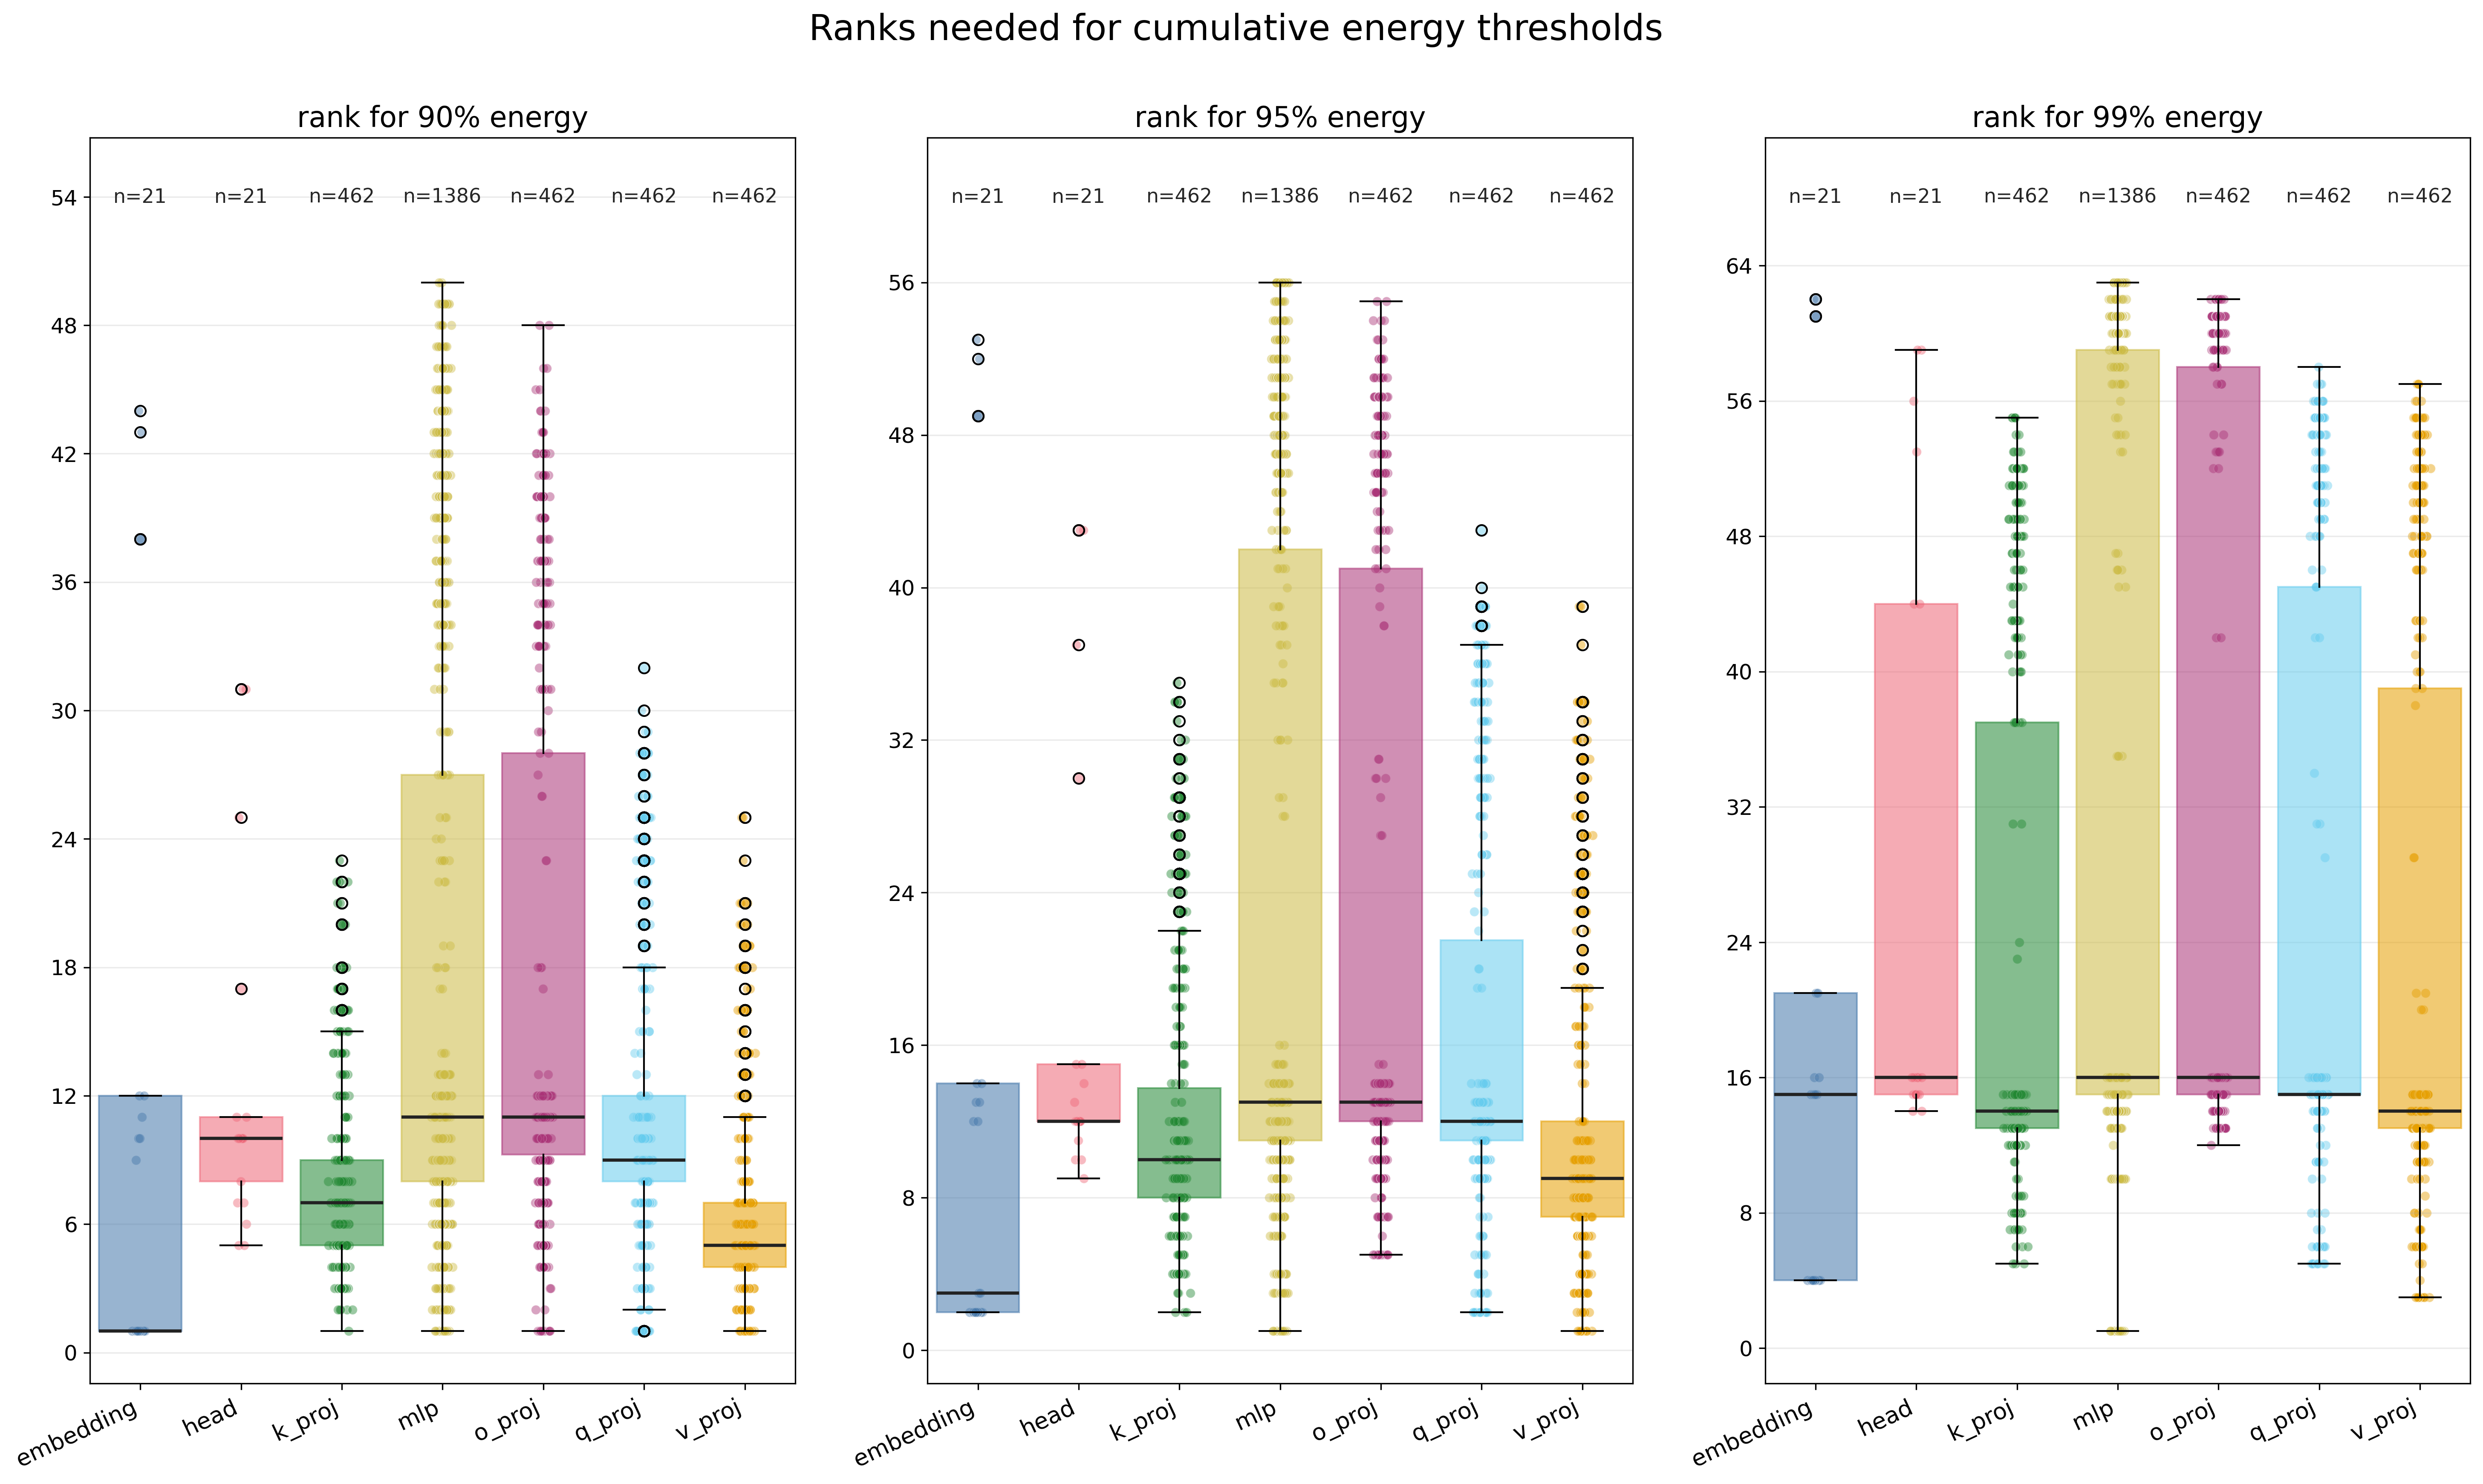
\includegraphics[width=0.9\textwidth]{figures/spectrum_group_threshold_rank_boxplots.png}
    \caption{Boxplots of ranks needed to capture 90\%, 95\%, and 99\% of the cumulative energy of the gradient's singular spectrum. Different layer groups (embedding, head, attention projections, MLP) exhibit widely varying spectral decay rates.}
    \label{fig:threshold_ranks}
\end{figure*}

Several observations can be made:

\begin{itemize}
    \item For the 90\% energy threshold, most layers require a rank between 2 and 6. This suggests that a fixed \(r=8\) is often unnecessarily large for many layers, wasting computational resources.
    \item For the 95\% threshold, the required rank increases noticeably, especially for \(q\_proj\), \(k\_proj\), \(v\_proj\), and MLP layers, where the median rank approaches 6--8. Some layers even require ranks above 10, indicating that the spectrum decays slowly.
    \item For the 99\% threshold, many layers require ranks significantly larger than 8 (up to 15--20 for some attention projections). This means that a low-rank approximation with \(r=8\) inevitably discards about 1\% of the gradient energy, which may affect convergence in the long term.
    \item The head and embedding layers consistently require very low ranks (often 1--2) to capture 90\% of the energy, confirming that these layers are nearly rank-deficient.
\end{itemize}

These findings provide a strong motivation for adaptive rank allocation: using a per-layer, dynamically adjusted rank that matches the spectral decay can save computation without sacrificing approximation quality. Our adaptive rank mechanism (Section~\ref{sec:implemented-algorithms}) was designed exactly for this purpose, though its benefit on the small 0.5\,GB dataset was not statistically significant.

\section{Future Work}

\subsection{Stochastic Subspace Sampling}
As an original extension of low-rank optimization, we propose moving away from the deterministic selection of strictly the top-$r$ singular values. Instead, we use a Stochastic Singular Vector Sampler (SSS), where projection rows are chosen probabilistically based on the magnitude of their singular values.

The motivation comes from the superposition hypothesis \cite{olah_superposition}: useful update directions may lie outside the dominant singular subspace. Our pilot runs on the 0.5\,GB subset gave a first positive signal---adaptive stochastic projection slightly outperformed deterministic GaLore2-mini and LOTUS-mini in validation perplexity---but the margin is small and the dataset is tiny, so this remains preliminary.

So far, SSS is implemented as a separate adaptive-stochastic variant. We have \emph{not} yet integrated it into the GaLore2-mini and LOTUS-mini code paths, and we have \emph{not} yet combined stochastic subspace selection with the randomized SVD used in GaLore2-mini. Closing these gaps is a concrete next step: the same sampler should plug into deterministic GaLore2 (random SVD + top-$r$), LOTUS (adaptive refresh + top-$r$), and their hybrid settings, so that all baselines are compared under one stochastic interface.

The open engineering questions for the sampler are:
\begin{enumerate}
    \item \textbf{Signal-to-noise separation:} filter small singular values that are mostly noise before sampling;
    \item \textbf{Temperature control:} adapt Softmax temperature to the current spectrum (e.g., via variance or coefficient of variation), balancing top-$r$ exploitation and controlled exploration.
\end{enumerate}

\subsection{Hyperparameter Tuning}
We have not yet performed a systematic search over method hyperparameters. At minimum, we plan a lightweight tuning pass before or alongside the full-dataset reruns: LOTUS threshold $\gamma$ and drift window, GaLore2 update gap and random-SVD oversampling, SSS temperature and $k_{\text{det}}$, adaptive-rank clamps, and learning-rate warmup length. The goal is not a full AutoML sweep, but a documented manual or small-grid adjustment so that comparisons on RefinedWeb are not locked to arbitrary first-try settings.

\subsection{Adaptive Rank Allocation}
Instead of a fixed rank $r$ across all layers, we continue the adaptive rank strategy already in the codebase. Our spectral analysis above shows that embedding and head layers often need very low rank, while some attention and MLP layers need more than $r=8$ even for 95\% energy capture. Per-layer ranks are set from the singular-value spectrum (energy + entropy). On the pilot dataset the benefit was not statistically significant; full-scale reruns and the tuning pass above may show whether layer-wise ranks improve the memory--quality trade-off at longer budgets.

\subsection{Full-Scale Validation}
The immediate experimental milestone is to rerun GaLore2-mini, LOTUS-mini, and stochastic variants on the full RefinedWeb corpus ($\approx$400\,GB) at batch size~16, sequence length~2048, and $32768$ tokens per step, then check whether any advantage of stochastic sampling or adaptive rank survives at scale.

\section{Schedule}

The remaining project work is scheduled from June~2 through June~14, 2026 (June~15 excluded).

\subsection{June 2--5: Full-scale reruns}
\begin{itemize}
    \item Rerun GaLore2-mini, LOTUS-mini, and the current adaptive-stochastic variant on the full RefinedWeb dataset ($\approx$400\,GB): batch size~16, sequence length~2048, $32768$ tokens per step, rank~$r=8$, seed~666, hyperparameters from Section~\ref{sec:experimental-setup}.
    \item Regenerate comparative tables, loss curves, and VRAM decomposition plots from the new logs.
\end{itemize}

\subsection{June 6--14: Integration, tuning, and follow-ups}
\begin{itemize}
    \item Integrate the stochastic sampler into the GaLore2-mini and LOTUS-mini projectors (not done in the pilot codebase).
    \item Combine stochastic subspace selection with randomized SVD in GaLore2-mini.
    \item Lightweight hyperparameter tuning ($\gamma$, update gap, SSS temperature, $k_{\text{det}}$, rank clamps, warmup).
    \item Further ablations, extra seeds, report/poster updates---exact scope to be fixed after the June~2--5 reruns.
\end{itemize}

By the end of this project, we will deliver the following outputs:
\begin{itemize}
    \item An open-source repository containing the implementations of 'LOTUS-mini', the stochastic sampler, the adaptive rank allocator, and the custom scheduler.
    \item Comprehensive comparative tables and learning curves illustrating the trade-offs between peak memory, training speed, and perplexity across all evaluated methods.
    \item An empirical comparison of stochastic singular vector sampling and adaptive layer-wise ranks against deterministic greedy selection on the full RefinedWeb rerun.
\end{itemize}

\bibliographystyle{IEEEtran}
\bibliography{literature}

\end{document}
